\documentclass[tikz,border=15pt]{standalone}
\usepackage{amsmath,amssymb}
\usetikzlibrary{calc}

\begin{document}
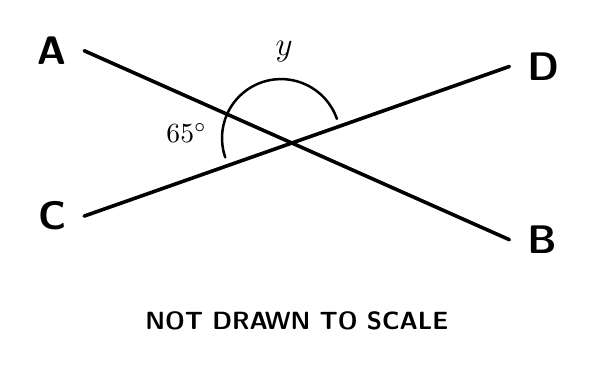
\begin{tikzpicture}[line cap=round, line join=round, scale=1.0]
  % Intersecting lines AB and CD
  \coordinate (A) at (0.2, 2.9);
  \coordinate (B) at (5.6, 0.5);
  \coordinate (C) at (0.2, 0.8);
  \coordinate (D) at (5.6, 2.7);

  % Intersection point O
  \coordinate (O) at (2.7, 1.79);

  % Lines
  \draw[line width=1.3pt] (A) -- (B);
  \draw[line width=1.3pt] (C) -- (D);

  % Angles
  % Angle 65 between OA and OC
  \draw[line width=0.9pt] ($(O) + (156:0.75)$) arc (156:199:0.75);
  \node[font=\normalsize] at ($(O) + (177:1.2)$) {$65^\circ$};

  % Angle y between OA and OD
  \draw[line width=0.9pt] ($(O) + (19:0.75)$) arc (19:156:0.75);
  \node[font=\large] at ($(O) + (88:1.1)$) {$y$};

  % Labels
  \node[left=3pt, font=\Large\sffamily\bfseries] at (A) {A};
  \node[right=3pt, font=\Large\sffamily\bfseries] at (B) {B};
  \node[left=3pt, font=\Large\sffamily\bfseries] at (C) {C};
  \node[right=3pt, font=\Large\sffamily\bfseries] at (D) {D};

  % Footer
  \node[below=14pt, font=\small\sffamily\bfseries] at (2.9, 0.2) {NOT DRAWN TO SCALE};

\end{tikzpicture}
\end{document}
